% !TEX root = ../main.tex

\chapter{Paper reproduction}
\label{ch:paper_reproduction}
This chapter relies on the article "Computer-Aided Diagnosis of Prostate Cancer Using a Deep Convolutional Neural Network from Multiparametric MRI"\cite{07} presented in chapter \ref{ch:literature_review}. It aims at reproducing the experiment of the paper in order to acquire the medical, theoretical and technical background before proposing a new transfer learning method as a way to improve the classification using other body parts and to overcome the lack of available data(see \ref{ch:transfer_learning}).\\

Furthermore, since the article does not provide the results their model got on the PROSTATEx challenge, the reproduction of the experiment can act like a benchmark to evaluate the generalization of the model to unseen data. 

\section{Process overview}
Schematically, the entire experiment process can be represented as shown in figure \ref{fig:paper_reproduction_process}. The PROSTATEx dataset is composed of samples whose clinical significance is provided (labeled data) and samples without this information (unlabeled data). The latter are used for the challenge, which consists in predicting the probability of patients lesions to be malignant (class 1) or benign (class 0). In both cases, the data is processed before been used (see \ref{prostatex_data_processing} for details). After the processing, the labeled data are split into training, validation and test sets using respectively 80\%, 10\% and 10\% of all available data for each set. The training set is then given in batches as input to the neural network, which update its weight consequently. At the end of each epoch, the current model is tested on the validation set (that the model has never seen previously) and the metrics are plotted on Tensorboard (see \ref{paper_tensorboard}). If the current model has a bigger AUC and a bigger accuracy than the previous best model, it becomes the best model and it is saved.  When the training phase reaches the defined number of epochs, the model is then tested on the test set. This same model is also used to take part into the PROSTATEx challenge in order to output predictions into a .csv file for each patient and findings.

\begin{figure}[!h]
\centering
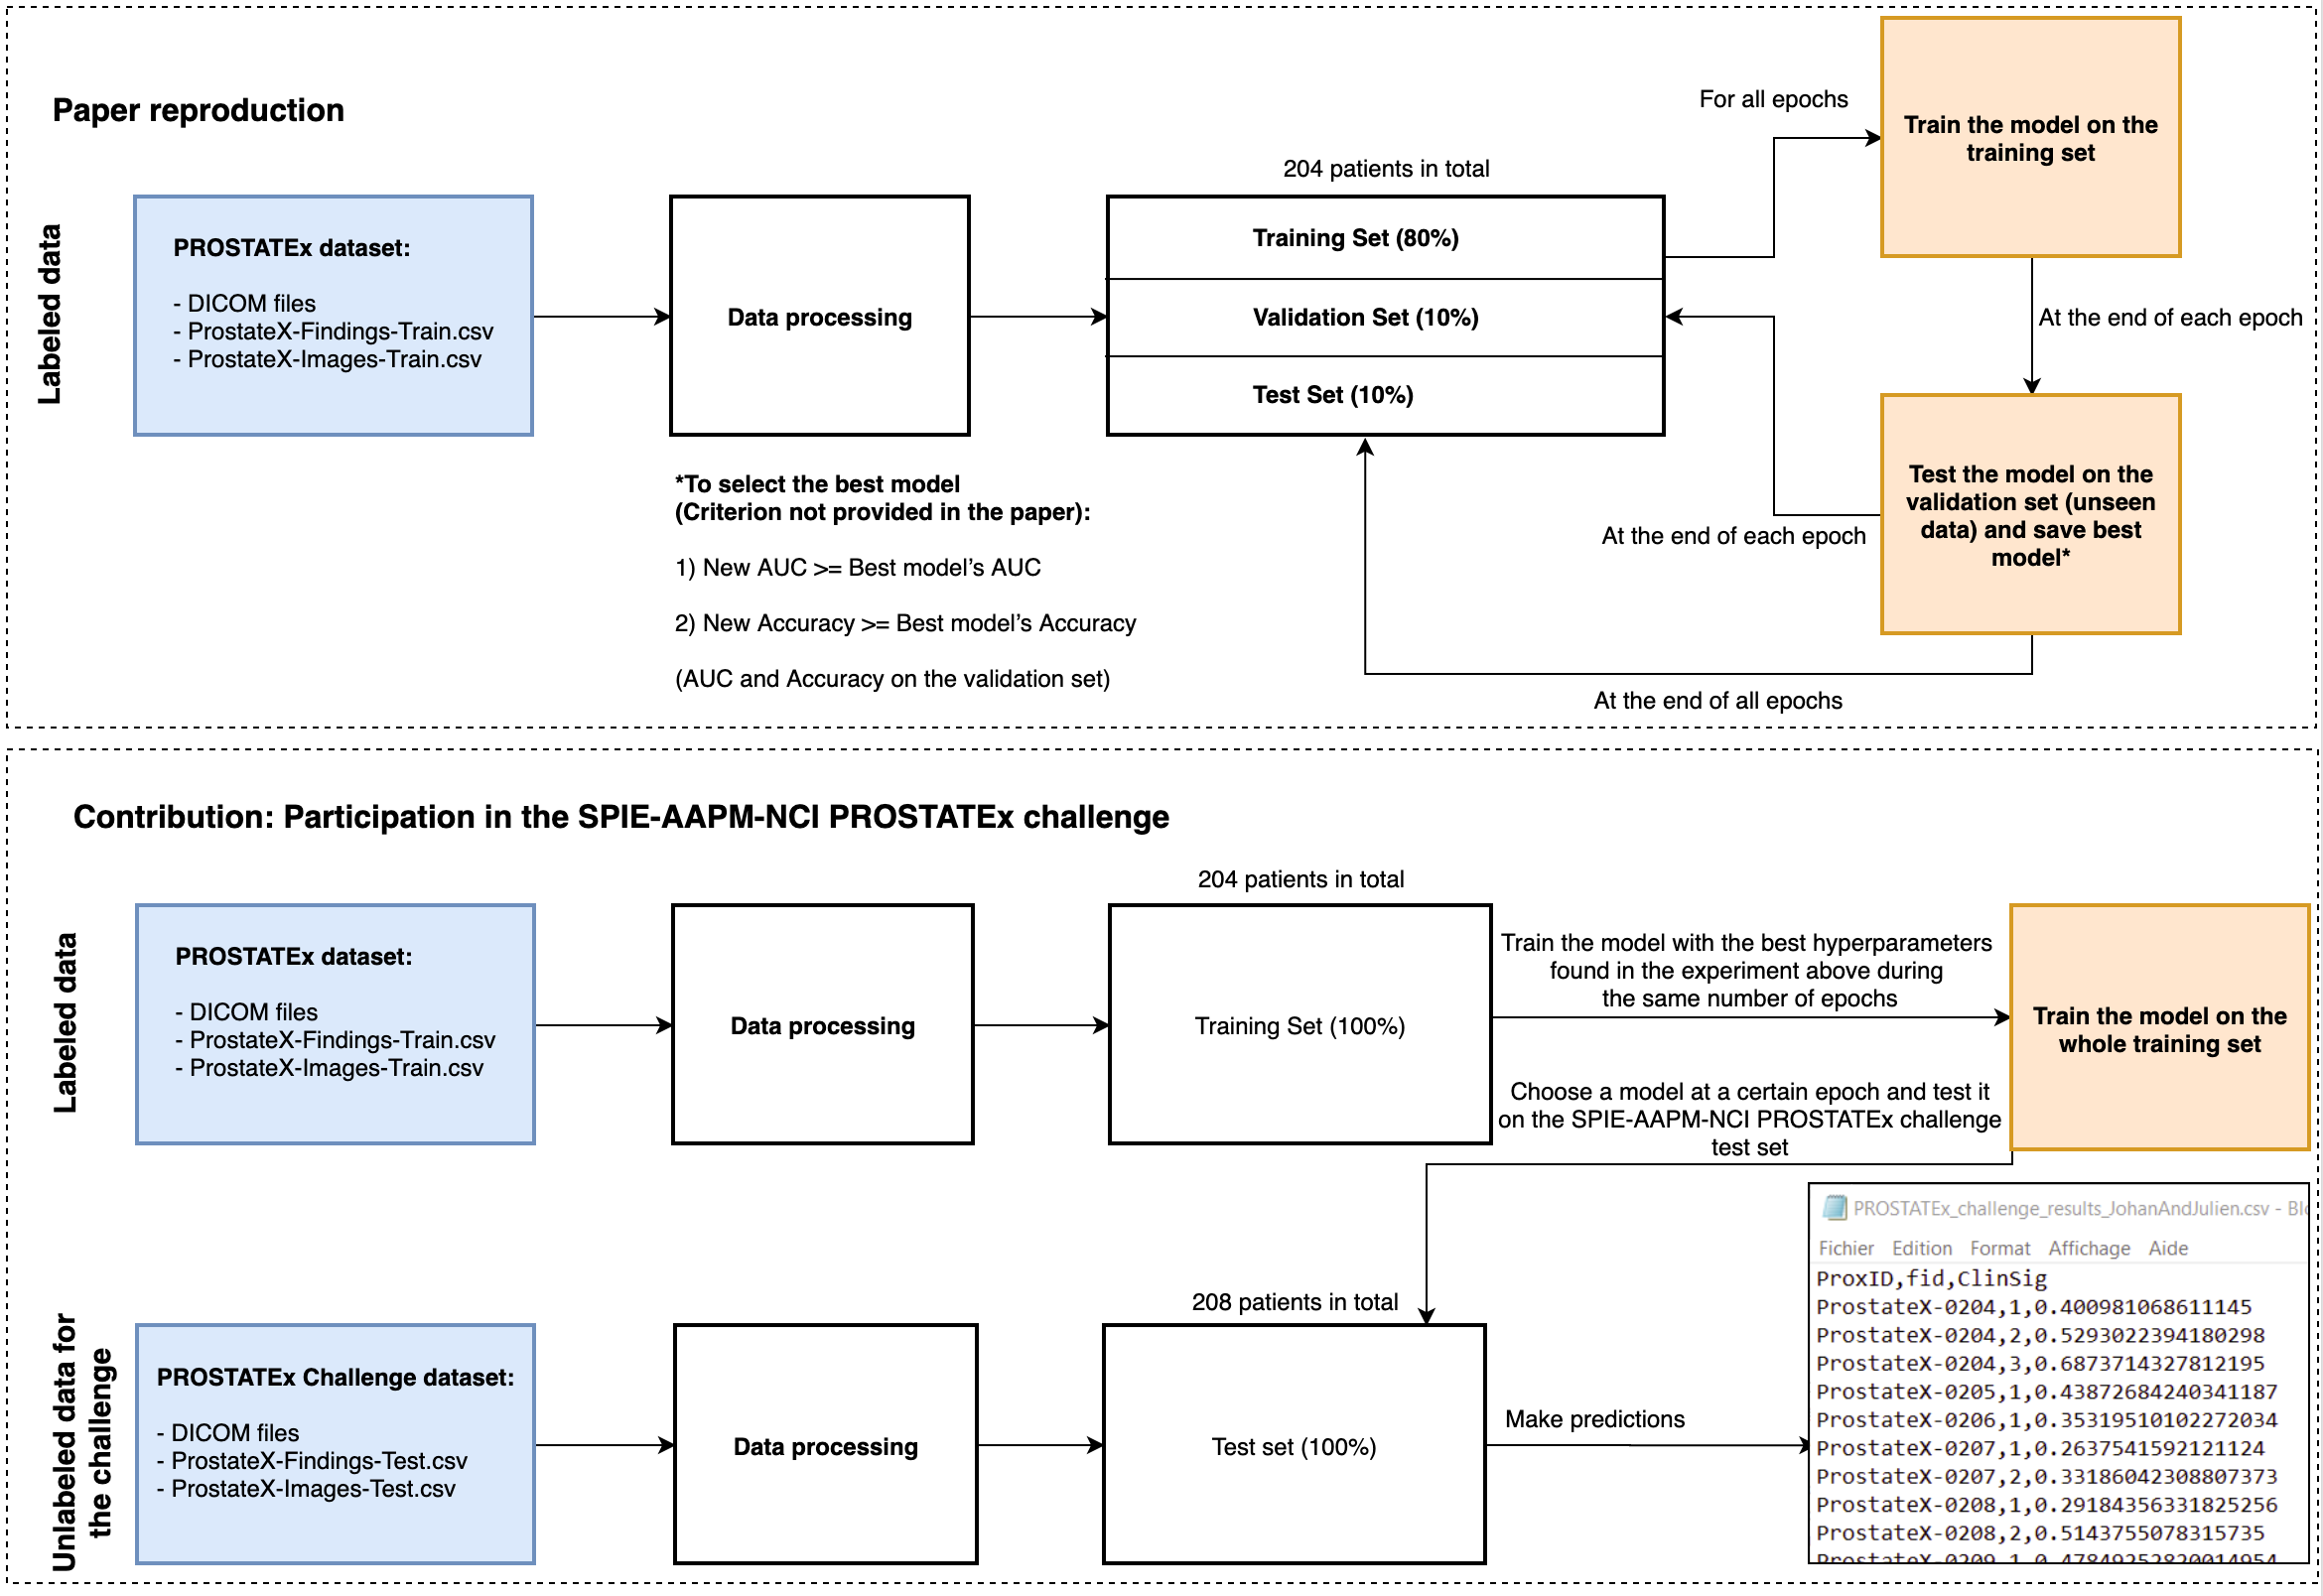
\includegraphics[width=1\textwidth, keepaspectratio=true]{./figures/paper_reproduction_process.png}
\caption{Paper reproduction experiment}
\label{fig:paper_reproduction_process}
\end{figure}


\section{PROSTATEx: Data processing}
\label{prostatex_data_processing}
\subsection{Dataset description}
\label{prostatex_dataset_description}
\subsection{From DICOM to NumPy arrays}
\subsection{From NumPy arrays to augmented stacked images}
\subsection{From NumPy arrays to augmented non-stacked images}
\subsection{Data processing verification}
\subsubsection{Cropping verification using red dots}
\subsubsection{Alignment visualization}

\section{Training the neural network}
\subsection{Architecture}
\subsection{Criterion to save the best model}
\subsection{Tensorboard}
\label{paper_tensorboard}
\subsection{Script options}
\subsection{Experimental setup}
\subsection{Training verification}
\subsubsection{Gradient flow visualization}

\section{Results}

\section{Discussion}